\chapter{Proposed Solution}
\label{chpt:5}

\paragraph{}
% In our framework, a machine comprehension model sees a question-context pair and is tasked with selecting the answer span in the passage, or responding \texttt{NIL} in case the answer is not present. The answer is the entity that is in relation with the entity in the question. 
In this Chapter we will present the different parts of our setup. We will start introducing the word representation models we used in Section~\ref{sec:w_e}; next, in Section~\ref{sec:namanda} the reading comprehension model and in Section~\ref{sec:xlingual} and \ref{sec:onemodel} we will describe the proposed architectures to benchmark the generalization abilities of the model by performing zero-shot experiments, both using unseen entities and unseen relations.


\section{Word Representation}
\label{sec:w_e}
\paragraph{}
We describe the two methods for word representation that we will compare: BERT and fastText. These model are used in the multilingual version, obtained using different techniques.

\subsection{BERT}
\paragraph{}
Proposed by~\cite{devlin2018bert}, BERT (Bidirectional Encoder Representations from Transformers) is a model for language representation. Similarly to~\citep{radford2018improving}, BERT uses a multi-layer transformer, with the addition that the transformer is bidirectional. The input representation is a sum over the token embedding, the position embedding, and the segment, which is the sentence encoding (the same for each token). BERT is pre-trained using as objective a Masked Language Model (MLM) and a next sentence prediction task. The MLM is based on the Cloze task \citep{taylor1953cloze}, the model is trained to predict the missing words that were randomly removed. This allows BERT to truly obtain a bidirectional representation. However, the use of a token to hide the word to predict creates discrepancies between the pretrain and the fine-tuning. Moreover, BERT assumes that the predicted token is independent from the other unmasked tokens, which ignores the high-order dependencies in natural languages~\citep{yang2019xlnet}.


The multilingual version has a shared embedding space for the top 100 languages with the largest Wikipedias. The entire Wikipedia dump for each language was taken as the training data for each language. The multilingual model has 12-layer, the internal hidden representation is of size 768, 12 attention heads, and a total of 110M parameters.

\subsection{fastText}
\paragraph{}
fastText~\citep{bojanowski2016enriching} learns $n$-grams representation and, using these representation, creates words representation as a sum of the $n$-grams is made of. fastText is based on the skip-gram with negative sampling model~\citep{mikolov2013distributed}, but with the use of subword information. In the negative sampling function (Equation~\ref{eq:neg_samp}), instead of using just the context word vector $\mathbf{\tilde{w}}_{t+j}$, we use the subword information. Given a word $x$, $G_x \subset \{1, \dots, G\}$ is the set of $n$-grams appearing in $x$. Each $n$-gram $g$ has a corresponding vector representation $\mathbf{z}_{g}$. Thus, we obtain the SG model with negative sampling and subword information:  

\begin{equation}
P\left(x_{t+j} | x_{t}\right)=\log \sigma\left( \sum_{g \in \mathcal{G}_{x_{t+j}}} \mathbf{z}_{g}^{\top} \mathbf{w}_{t}\right)+\sum_{i=1}^{k} \mathbb{E}_{w_{i} \sim P_{z}} \log \sigma\left(- \sum_{g \in \mathcal{G}_{x_{t+j}}} \mathbf{z}_{g}^{\top}\mathbf{w}_{t}\right)
\end{equation}

Using the $n$-grams allows to better model morphological rich languages such as Finnish, and Turkish since even rare morphological inflections are modeled. Moreover, using $n$-grams allows to model unseen words since we can just sum the representation of the $n$-grams is made of. 

The multilingual embeddings we use are obtained by training independent vector representations using fastText on each language's Wikipedia and common crawl corpora, then using a solution similarly to~\citep{mikolov2013exploiting} (Equation~\ref{eq:word_alignment}) the words are aligned into a common space. 

\section{NAMANDA}
\label{sec:namanda}
\paragraph{}
Previous neural models for reading comprehension based question answering \citep{seo2016bidirectional, yang2017words} focus on context-question interaction to capture similarities to extract the answer span. However, they don't model the question/answer type and also are unsuccessful to aggregate information from multiple sentences. AMANDA~\citep{kundu2018amanda} (An end-to-end question-focused Multi-factor Attention Network for Document-based question Answering), and the nil-aware version NAMANDA~\citep{kundu2018namanda} solve the previous issues by using a multi-factor attentive encoding based on tensor transformation and a max-attentional question aggregation mechanism to learn the meaningful pars of the question. 

AMANDA and NAMANDA share the same structure with the only difference in the answer layer, where NAMANDA adds the possibility for unanswerable question. We describe NAMANDA (Figure~\ref{fig:namanda}) by grouping the different layers into the general structure of reading comprehension models~\citep{qiu2019survey}.  

\begin{figure}[h]
\centering
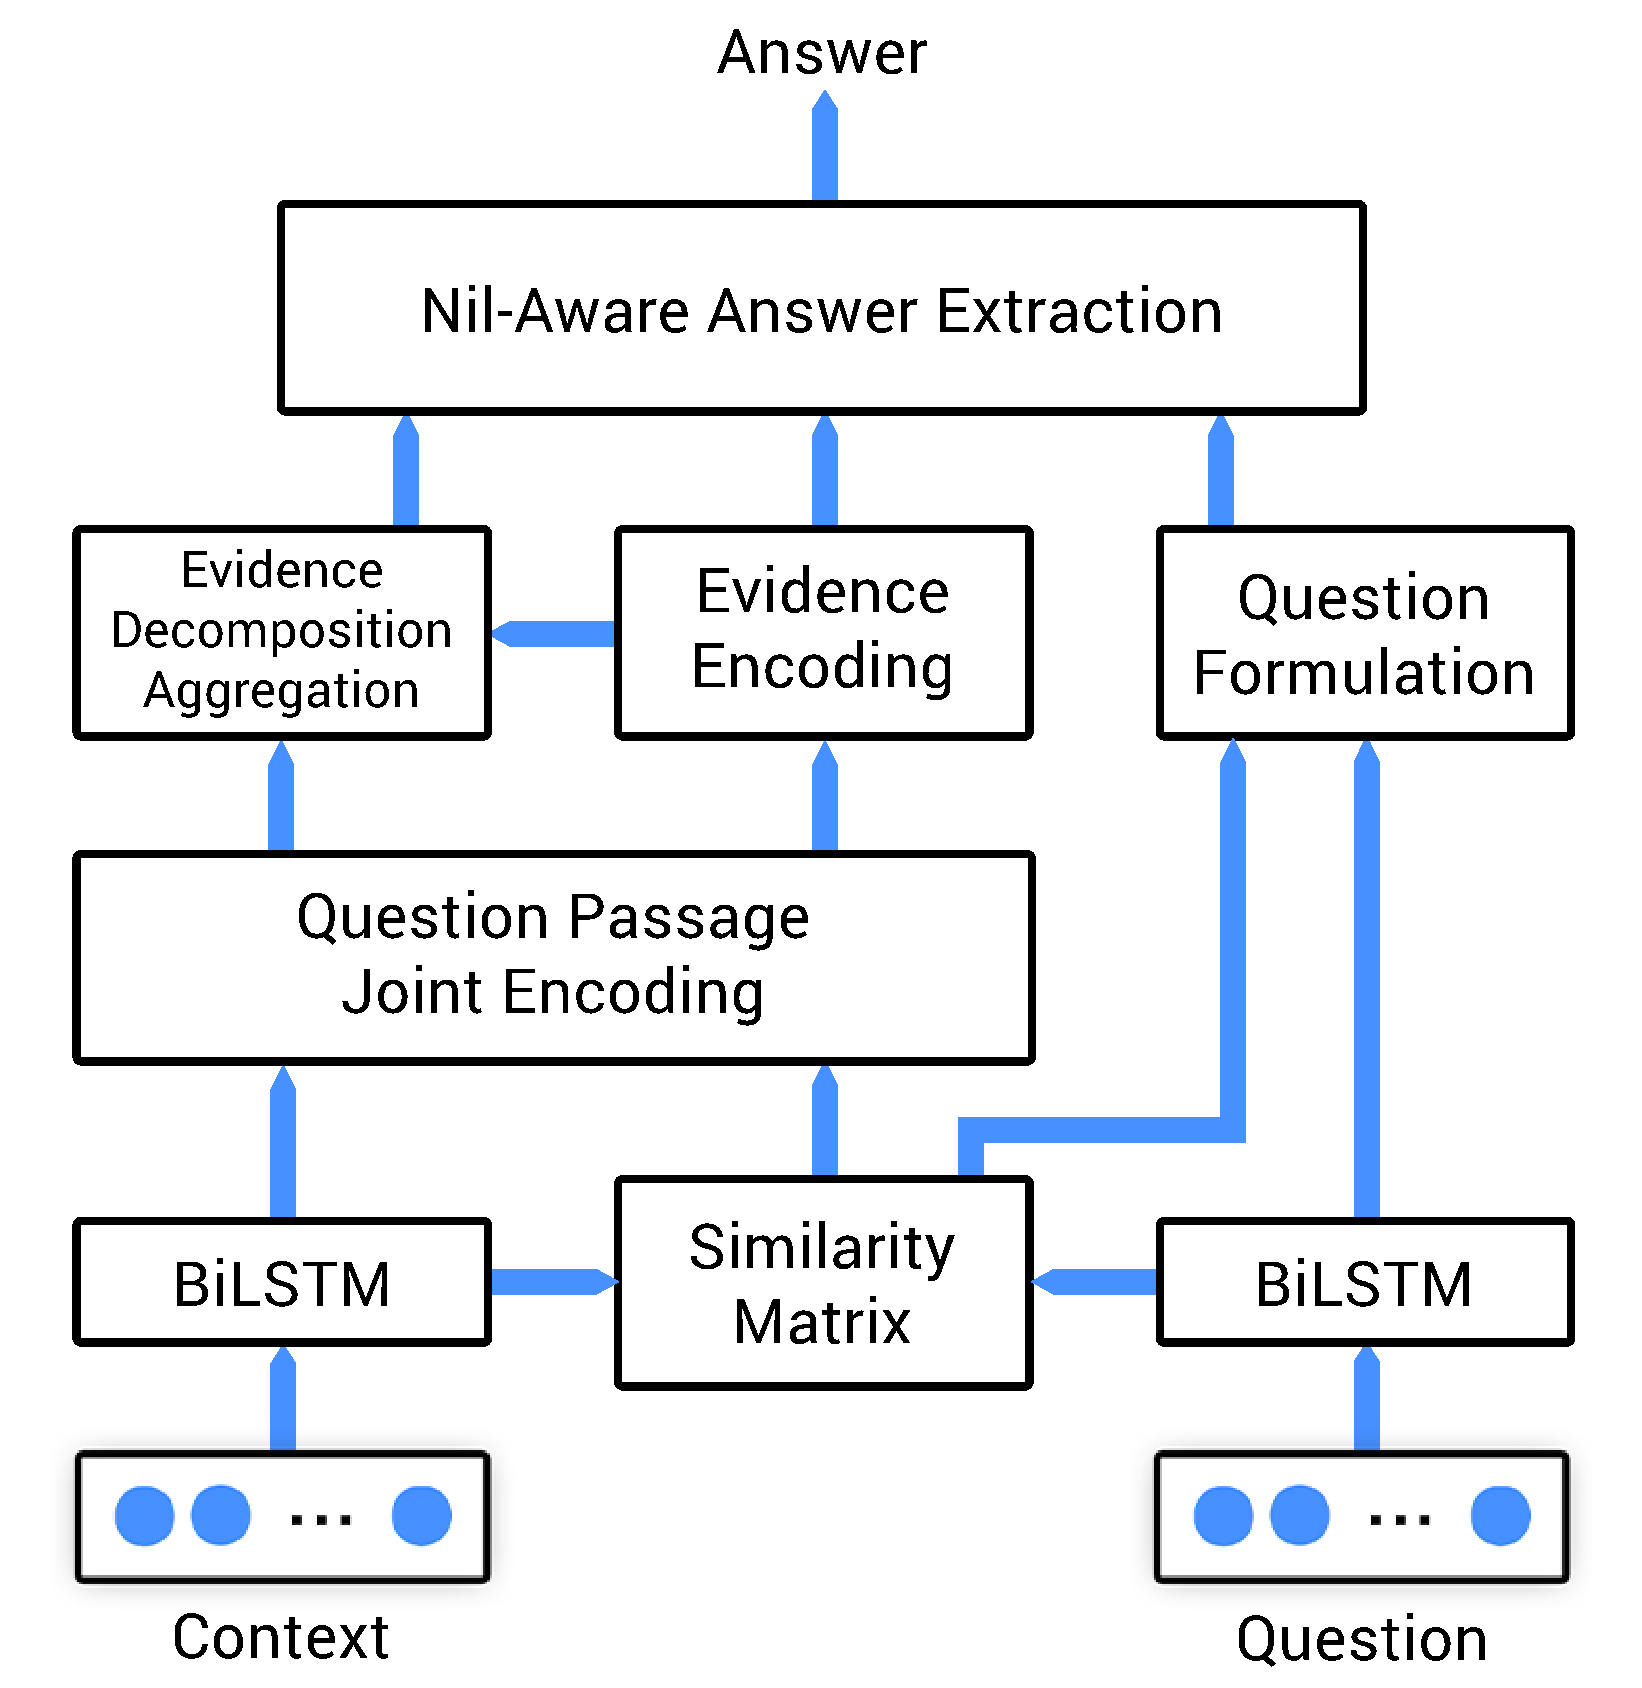
\includegraphics[width=0.4\textwidth]{images/namanda.pdf}
\caption{An overview of NAMANDA's architecture.}
\label{fig:namanda}
\end{figure}


\subsubsection{Embed Layer}
NAMANDA uses word-level embedding by concatenating the word embeddings from GloVe~\citep{pennington2014glove} and a CNN based character embedding. Using character embedding is useful for out-of-vocabulary words. In our experiments we will use different embeddings.

\subsubsection{Encoding Layer}
To encode the contextual information in the context and the question, a BiLSTM is used. Given a  context $c=\{c_1,\dots,c_T\}$ and a query $q=\{q_1, \dots, q_T\}$, we fed them into two separate LSTMs obtaining $\mathbf{P} \in \mathbb{R}^{T \times d}$, and $\mathbf{Q} \in \mathbb{R}^{U \times d}$, with $d$ the number of hidden units. The rows of these matrix is the concatenation of the forward and the backward hidden state at each time step.

\newpage

\subsubsection{Match Layer}
NAMANDA has various layers that help performing the match, these are:
\begin{itemize}[-]
    \item \textbf{Similarity Matrix}: it express the similarity between the words in the passage and the words in the question. The similarity matrix $\mathbf{A} \in \mathbb{R}^{T \times U}$ is defined as $\mathbf{A} = \mathbf{D}\mathbf{Q}^{\intercal}$.
    \item \textbf{Question Formulation}: the most relevant parts of the question are extracted using  \begin{enumerate*} [a) ]
        \item a max-attentional question aggregation ($q_{ma})$
        \item a question type representation ($q_f$).
    \end{enumerate*} The important parts of the question are aggregated in $q_{ma} = k\mathbf{Q}$, where $k = softmax_{col}(A)$. The question type is encoded as a concatenation of the first \textit{``Wh"} word $q_{t_{wh}}$, and its following word $q_{t_{wh}+1}$ (the $t_{wh}$-th, and $(t_{wh}+1)$-th rows of $\mathbf{Q}$), $q_f = [q_{t_{wh}}, q_{t_{wh}+1}]$. The final question representation computed using a feed-forward network $\tilde{q} = {FF}([q_{ma}, q_f]; W_q)$. 
    
    \item \textbf{Question-Passage Joint Encoding}: the encoding is achieved using a row-wise softmax over the similarity matrix $\textbf{R} = softmax_{row}(\mathbf{A})$. The rows in $\mathbf{R}$ measure how relevant the words in the question are w.r.t the context. The aggregated question representation $\mathbf{G} \in \mathbb{R}^{T \times d}$ is computed as $\mathbf{G} = \mathbf{R}\mathbf{Q}$. The concatenation of the aggregated question vectors and the passage encoding are concatenated in $\mathbf{S} \in \mathbb{R} ^{T \times 2d}$, then a BiLSTM is applied obtaining  $\mathbf{V} \in \mathbb{R} ^{T \times d}$.
    
    
    \item \textbf{Evidence Decomposition Aggregation}: The information between multiple sentence is aggregated using a multi-factor attentive encoding using tensor-based transformation. This allows to collect information at different grain level for long contexts.
    Given the number of factors $m$, the multi-factor attention $\mathbf{F}^{[1:m]} \in \mathbb{R} ^{T \times m \times T}$ is formulated as:
    
    \begin{equation}
    \mathbf{F}^{[1:m]} = \mathbf{V}\mathbf{W}_{f}^{[1:m]}\mathbf{V}^{\intercal}    
    \end{equation}
    
    where $\mathbf{W}_{f}^{[1:m]} \in \mathbb{R} ^{d \times m \times d}$ is a 3-way tensor. The evidence are refined using a max-pooling over the factors, a self-attention matrix $\mathbf{F} \in \mathbb{R} ^{T  \times T}$ is obtained. $\mathbf{F}$ is further processed using a row-wise softmax obtaining $\mathbf{\tilde{F}}$. Then the self-attentive encoding is $\mathbf{M} = \mathbf{\tilde{F}}\mathbf{V}$, with $\mathbf{M} \in \mathbb{R} ^{T \times H}$. The self-attentive encoding is concatenated with the question-dependent passage, and then a feed-forward neural network-gating is applied, obtaining $\mathbf{Y}$, with $\mathbf{Y} \in \mathbb{R}^{T \times 2d}$.
    
    
    Following~\citep{wang-etal-2016-sentence}, the evidence vectors for each context word are decomposed using orthogonal decomposition. Each row $y_t$ of $\mathbf{Y}$ is decomposed with respect to the question-passage joint encoding ($\mathbf{S}$) vector $s_t$ into its parallel components $y_{t}^{=}$, which represent the relevant parts of the accumulated evidence, and perpendicular components $y_{t}^{\perp}$ that represent the irrelevant parts.
    
    \begin{equation}
        y_{t}^{=}=\frac{y_{t} s_{t}^{\top}}{s_{t} s_{t}^{\top}}s_{t}
    \end{equation}
    
    \begin{equation}
        y_{t}^{\perp}=y_{t}-y_{t}^{=}
    \end{equation}
    
    The aggregation step is performed applying a feed-forward network over the previous components, and obtaining the matrix $\mathbf{Y}^a$, where the rows are:
    
    \begin{equation}
        y_{t}^{a} = FF\left(\begin{bmatrix}
           y_{t}^{=} \\
           y_{t}^{\perp}
         \end{bmatrix}; W_a\right)
    \end{equation}
    
    Then a max-pooling operation over all words in $\mathbf{Y}^a$ is applied to obtain the \texttt{NIL} vector representation $\hat{n}$. Finally, a nil pointer score $n_s$ is computed using a learnable weight $w_{n}^{\intercal}$, having $n_s = \hat{n}\textbf{w}_{n}^{\intercal}$. The nil pointer score will be used to normalize the start and end pointer.
    
\end{itemize}

\subsubsection{Answer Layer}
NAMANDA uses a two stacked BiLSTMs on $\mathbf{Y}$ to determine the beginning and the end of the answer span. The hidden representations of these LSTMs are $\mathbf{B} \in \mathbb{R}^{T \times d}$, and $\mathbf{E} \in \mathbb{R}^{T \times d}$. The scores for the beginning $s_b$, and the end $s_e$, are then calculated using the question vector $\tilde{q}$, and the output of the stacked BiLSTMs $\mathbf{B}$, and $\mathbf{E}$.

\begin{equation}
s_b = \tilde{q} \, \mathbf{B}^{\intercal}
   \quad\mathrm{and}\quad 
s_e = \tilde{q}\, \mathbf{E}^{\intercal}
\end{equation}

Now, the \texttt{NIL} score is prepended, obtaining $\hat{s_b} = [n_s, s_b]$ and $\hat{s_e} = [n_s, s_e]$. The final spans are:

\begin{equation}
\begin{split}
    P(b | c, q) & = softmax(\hat{s_b}) \\
    P(e | c, q) & = softmax(\hat{s_e})
\end{split}
\end{equation}

And the answer joint probability is:

\begin{equation}
    P(a|c, q) = P(b | c, q)P(e | c, q)
\end{equation}

The \texttt{NIL} label is assigned when $b=1$.

\section{Architectures}
\paragraph{}
In addition to using a monolingual nil-aware QA model, we use two architecture to evaluate the use of a multilingual resource for the relation extraction task. The first is a fine-tuning setup, the second is a multi-task learning. These model will be evaluated on two scenarios to find if the zero-shot relation extraction also benefits from our multilingual resource. 

\subsection{Cross-lingual Model Transfer}
\label{sec:xlingual}
\paragraph{}
This setup (Figure~\ref{fig:setupTransfer}) is used to see how well RE models can be transferred across languages. In this scenario, the first language has more data, while the target language is a low resource one. The knowledge transfer is aided by the use of a multilingual word representation.

The first step is to pretrain the model on the source language. Then, in the second step, the model is finetuned using the examples in the target language. The fine-tuning is performed on the entire model except for the embeddings which are kept frozen.

\begin{figure}[h]
    \centering
    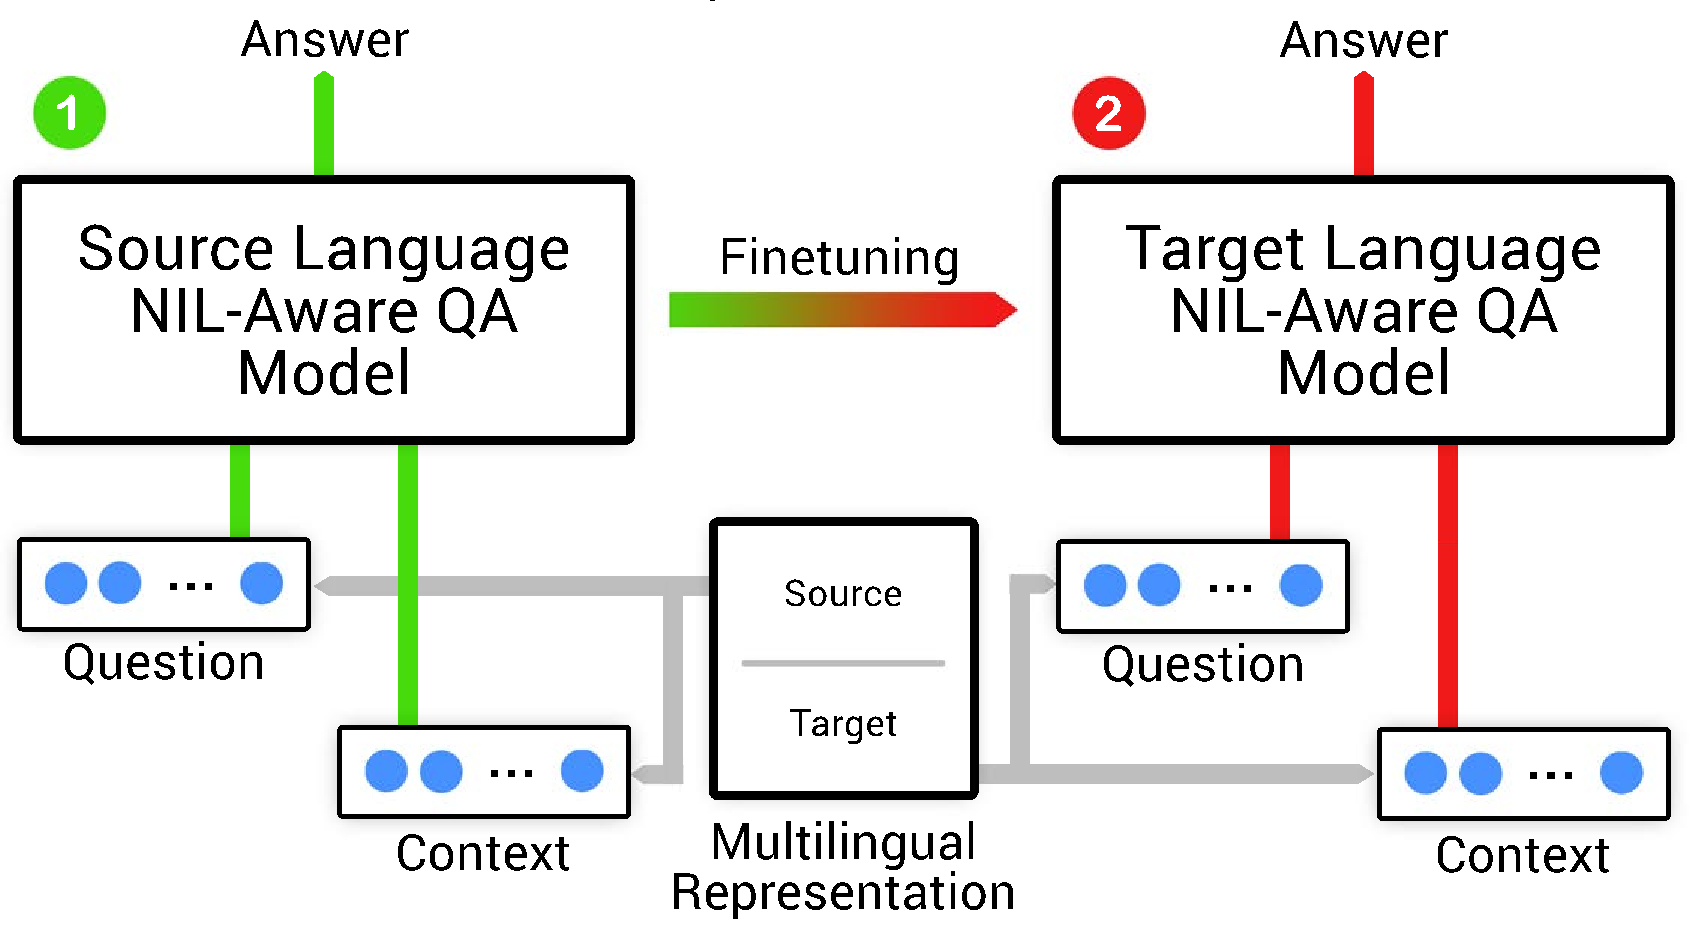
\includegraphics[width=0.7\textwidth]{images/model_v2.pdf}
    \caption{Cross-lingual model transfer. In step (1), a source language model is trained until convergence. In step (2), it is finetuned on a limited amount of target language data.}
    \label{fig:setupTransfer}
\end{figure}%

\subsection{One Model, Multiple Languages}
\label{sec:onemodel}
\paragraph{}
Shown in Figure~\ref{fig:setupMulti}, this setup trains a single model using multiple languages. This model test the ability of a single model to perform RE across multiple languages. In this architecture, the network is trained to maximize the objective function of all languages jointly. Beside of the benefits of MTL, the model is also using the signal from other languages to better generalize unseen entities or relation in a specific languages.



\begin{figure}[h]
    \centering
     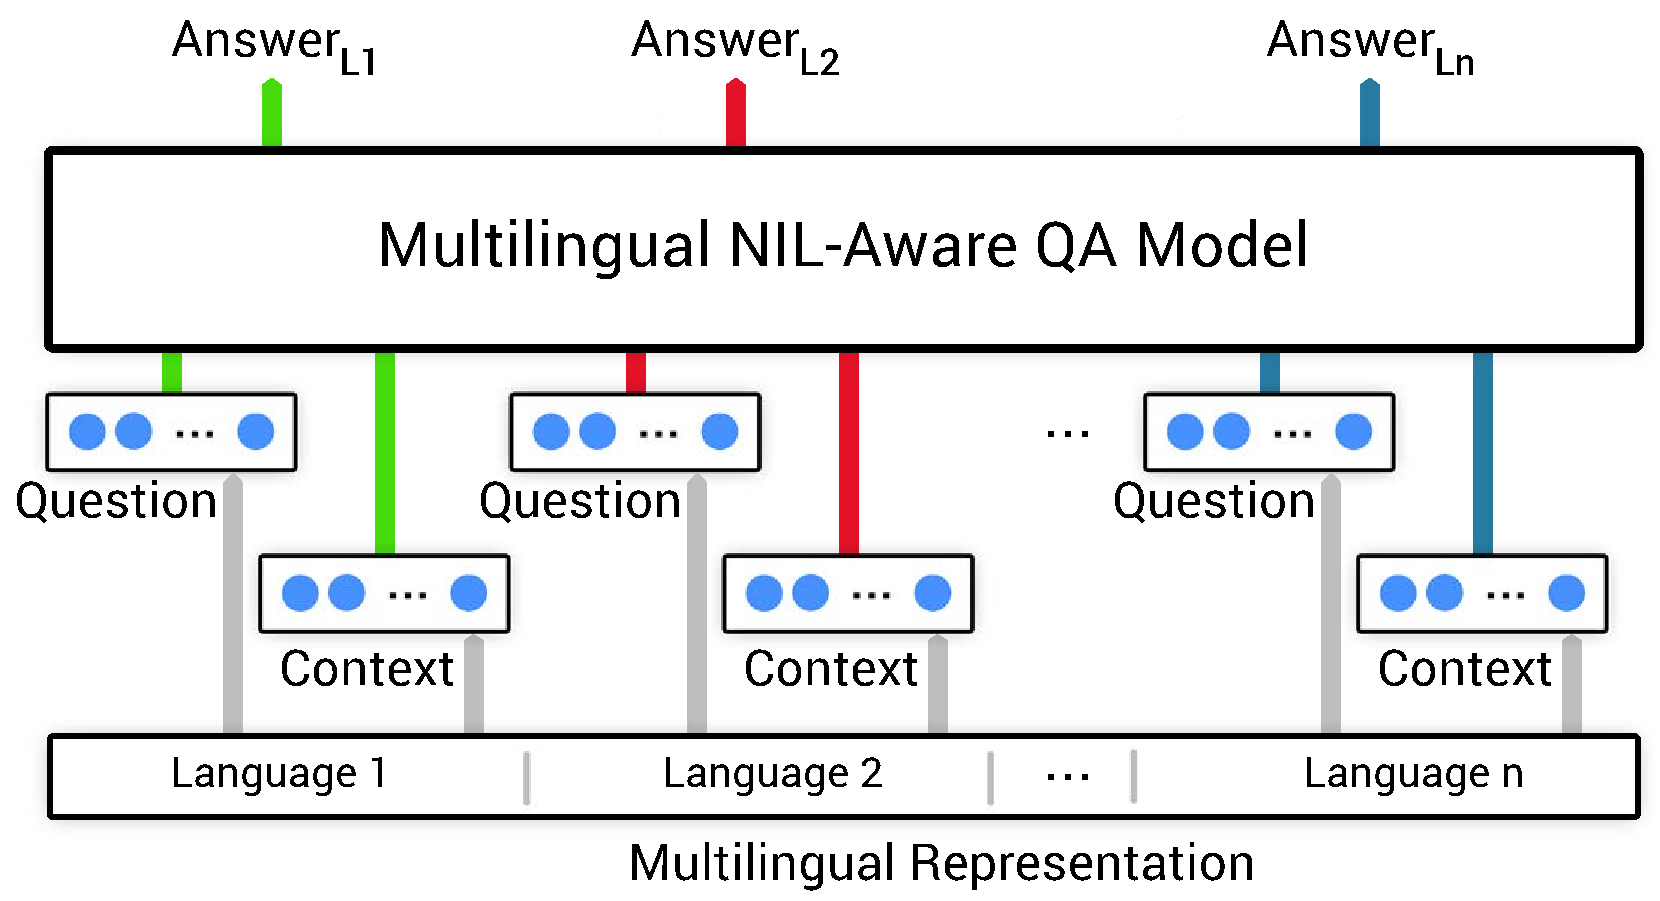
\includegraphics[width=0.7\textwidth]{images/model_joint_unique.pdf}
    \caption{Joint multilingual training.}
    \label{fig:setupMulti}
\end{figure}